\documentclass[ignorenonframetext,]{beamer}
\setbeamertemplate{caption}[numbered]
\setbeamertemplate{caption label separator}{: }
\setbeamercolor{caption name}{fg=normal text.fg}
\beamertemplatenavigationsymbolsempty
\usepackage{lmodern}
\usepackage{amssymb,amsmath}
\usepackage{ifxetex,ifluatex}
\usepackage{fixltx2e} % provides \textsubscript
\ifnum 0\ifxetex 1\fi\ifluatex 1\fi=0 % if pdftex
  \usepackage[T1]{fontenc}
  \usepackage[utf8]{inputenc}
\else % if luatex or xelatex
  \ifxetex
    \usepackage{mathspec}
  \else
    \usepackage{fontspec}
  \fi
  \defaultfontfeatures{Ligatures=TeX,Scale=MatchLowercase}
\fi
% use upquote if available, for straight quotes in verbatim environments
\IfFileExists{upquote.sty}{\usepackage{upquote}}{}
% use microtype if available
\IfFileExists{microtype.sty}{%
\usepackage{microtype}
\UseMicrotypeSet[protrusion]{basicmath} % disable protrusion for tt fonts
}{}
\newif\ifbibliography
\hypersetup{
            pdftitle={From Probability to Statistical Inference},
            pdfauthor={Leanne Dong},
            pdfborder={0 0 0},
            breaklinks=true}
\urlstyle{same}  % don't use monospace font for urls
\usepackage{longtable,booktabs}
\usepackage{caption}
% These lines are needed to make table captions work with longtable:
\makeatletter
\def\fnum@table{\tablename~\thetable}
\makeatother
\usepackage{graphicx,grffile}
\makeatletter
\def\maxwidth{\ifdim\Gin@nat@width>\linewidth\linewidth\else\Gin@nat@width\fi}
\def\maxheight{\ifdim\Gin@nat@height>\textheight0.8\textheight\else\Gin@nat@height\fi}
\makeatother
% Scale images if necessary, so that they will not overflow the page
% margins by default, and it is still possible to overwrite the defaults
% using explicit options in \includegraphics[width, height, ...]{}
\setkeys{Gin}{width=\maxwidth,height=\maxheight,keepaspectratio}

% Prevent slide breaks in the middle of a paragraph:
\widowpenalties 1 10000
\raggedbottom

\AtBeginPart{
  \let\insertpartnumber\relax
  \let\partname\relax
  \frame{\partpage}
}
\AtBeginSection{
  \ifbibliography
  \else
    \let\insertsectionnumber\relax
    \let\sectionname\relax
    \frame{\sectionpage}
  \fi
}
\AtBeginSubsection{
  \let\insertsubsectionnumber\relax
  \let\subsectionname\relax
  \frame{\subsectionpage}
}

\setlength{\parindent}{0pt}
\setlength{\parskip}{6pt plus 2pt minus 1pt}
\setlength{\emergencystretch}{3em}  % prevent overfull lines
\providecommand{\tightlist}{%
  \setlength{\itemsep}{0pt}\setlength{\parskip}{0pt}}
\setcounter{secnumdepth}{0}

\title{From Probability to Statistical Inference}
\author{Leanne Dong}
\date{03/09/2018}

\begin{document}
\frame{\titlepage}

\begin{frame}{Linear Combination of random variables}

\begin{itemize}
\item
  Quite Often, we are interested in a linear combination of random
  variable rather than just one single random variable.
\item
  Let \(X_1,X_2,\cdots,X_n\) be a sequence of independent random
  variables with \(\mathbb{E}X_i=\mu_i\) and
  \(\text{Var}X_i=\sigma^2_i\) for \(i=1,\cdots,n\).
  \[\mathbb{E}(\sum^n_{i=1}X_i)=\sum^n_{i=1}\mathbb{E}X_i\].
\end{itemize}

\[\text{Var}(\sum^n_{i=1}X_i)=\sum^n_{i=1}\text{Var}X_i\]

\end{frame}

\begin{frame}{Linear Combination of random variables: Example 1}

Let \(X\sim N(\mu=100,\sigma=15)\) and \(Y\sim N(\mu=30,\sigma=5)\) be
independent random variables. Find the distribution \(X-Y\).

\textbf{Solution}:

Let \(Z=X-Y=(1)X-(-1)Y\), so \(a_1=1\) and \(a_2=-1\).
\[\mathbb{E}Z=a_1\mu_x+a_2\mu_y=1\times 100+(-1)\times 30=70\]
\[\text{Var}(Z)=a^2_1\text{Var}X+a^2_2\text{Var}Y=1^2\times 15^2+(-1)^2\times 5^2=250\]

\end{frame}

\begin{frame}{Linear Combination of random variables: Example 2}

Let \(X_1,X_2, and X_3\sim N(\mu=9,\sigma=4)\) be independent random
variables. Fina the distribution of the mean of \(X_1,X_2\) and \(X_3\).

\textbf{Solution}:
\[\bar{X}=\frac{X_1+X_2+X_3}{3}=\frac{1}{3}X_1+\frac{1}{3}X_2+\frac{1}{3}X_3\]
\[\mathbb{E}\bar{X}=\frac{1}{3}\times 9+\frac{1}{3}\times 9+\frac{1}{3}\times 9=9\]

\begin{align*}
\text{Var}(\bar{X})&=(1/3)^2\times 4^2+(1/3)^2\times 4^2+(1/3)^2\times 4^2\\
&=\frac{16\times 3}{9}=\frac{16}{3}=\frac{4^2}{3}=\frac{\sigma^2}{n}
\end{align*}

\end{frame}

\begin{frame}{Distribution of the sums of normal Random variables and
sampling}

Given a sequence of independent random variables
\(X_i\sim N(\mu_i,\sigma^2_i)\) for \(i=1,\cdots,n\).
\[\sum^n_{i=1}a_i X_i\sim N(\sum^n_{i=1}a_i\mu_i,\sum^n_{i=1}a^2_i\sigma^2_2)\]

Given a sequence of independent and identically distributed (iid) random
variables \(X_i\sim N(\mu,\sigma^2)\) and constant \(a_i\) for
\(i=1,\cdot,n\)
\[\bar{X}=\frac{1}{n}\sum^n_{i=1}X_i\sim N(\mu,\frac{\sigma^2}{n}),\,\,\sum^n_{i=1}X_i\sim N(n\mu,n\sigma^2)\]

\end{frame}

\begin{frame}{Sample mean and variance}

\begin{itemize}
\item
  In view of the previous slide, if \(X\sim N(\mu,\sigma^2)\), then we
  know that the distribution of \(\bar{X}\) is
  \(N(\mu,\frac{\sigma^2}{n})\) for samples of size \(n\)!
\item
  If \(X\sim N(\mu,\sigma^2)\), then one can infer the distribution of
  the mean \(\bar{X}\), the mean of a sample of size \(n\).
\item
  More precisely, by some algebra,
  \[\mathbb{E}X=\mu\,\,\text{then}\,\,\mathbb{E}\bar{X}=\mu\]
  \[\text{Var}X=\sigma^2\,\,\text{then}\,\,\text{Var}(\bar{X})=\frac{\sigma^2}{n}\]
\item
  {The variability of the mean of a sample is less variable than the
  individual observations.} (Think why!)
\end{itemize}

\end{frame}

\begin{frame}{Sampling from a Normal Population}

\begin{itemize}
\item
  In the particular case of normal distribution, if
  \(X\sim N(\mu,\sigma^2)\), we know that the distribution of
  \(\bar{X}\) is \(N(\mu,\frac{\sigma^2}{n})\) for samples of size
  \(n\)!
\item
  Hence we can use all our knowledge of the normal distribution to apply
  to the distribution of the mean - only reducing the variance.
\end{itemize}

\end{frame}

\begin{frame}{Example: sampling from normal distribution}

Consider a population of male students which has a normal distribution
with mean height of \(176\) and a standard deviation of \(4\) cm. This
height \(X\sim N(176,16)\) is a random variable.

If a student were selected at random from that population the chance
they had a height between \(172\) cm and \(180\) cm would be
\(\mathbb{P}(172\le X\le 180)=0.6826\).

Suppose sets of 4 students were selected randomly and their mean height
\(\bar{X}\) was calculated. Then \(\bar{X}\sim N(176,4).\) and
\(\mathbb{P}(172\le X\le 180)\approx 0.9544\).

\end{frame}

\begin{frame}{Normal distribution (Review)}

\begin{itemize}
\item
  Surely the most frequently encountered continuous probability
  distribution is the so-called \emph{Normal distribution}. One reason
  is because it can be used to model the distribution of the errors
  arising in the measurement of many physical quantities.
\item
  The normal distributution can also be used to estimate discrete
  distributions (such as Poisson, Binomial) where sample size gets
  larger by a continuity correction.
\item
  On other hand, it plays a major role in statistical inference as we
  shall see.
\end{itemize}

\end{frame}

\begin{frame}{Normal distribution (Review)}

\begin{figure}
\centering
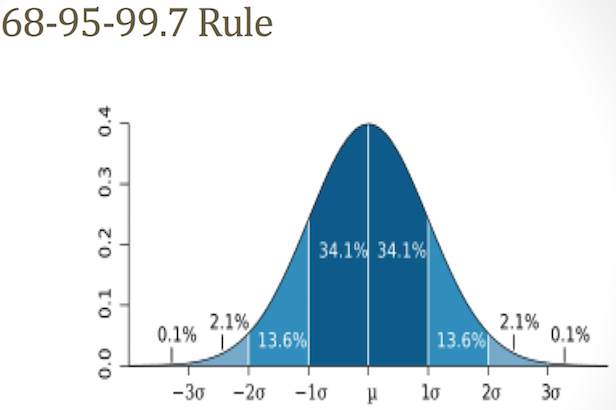
\includegraphics{68-95-99.png}
\caption{}
\end{figure}

\end{frame}

\begin{frame}{Approximation using Normals}

\begin{itemize}
\item
  Binomial
  \[X\sim\text{Bin}(n,p)\,\,\longrightarrow\,\,N(\mu=np,\sigma^2=np(1-p)\]
\item
  Poisson
  \[X\sim\text{Pois}(\lambda)\,\,\longrightarrow\,\,N(\mu=\lambda,\sigma^2=\lambda)\]
\end{itemize}

Moreover, one can improve the approximations using the
\textbf{continuity correction}, i.e.
\[\mathbb{P}(20\le X\le 22)\approx\mathbb{P}(19.5\le X\le 22.5)\]

\end{frame}

\begin{frame}{Continuity adjustment}

\begin{itemize}
\item
  When approximating a discrete distribution we must use the
  \emph{continuity correction} i.e.~as we cannot determine
  \(\mathbb{P}(X=3)\) directly, say, we calculate
  \(\mathbb{P}(2.5\le X\le 3.5)\).
\item
  Given a discrete integer valued r.v. \(X\sim (\mu,\sigma^2)\) and the
  approximating normal \(Y\sim N(\mu,\sigma^2)\) we adjust by 1/2 to
  (usually) improve the approximation.
  \[\mathbb{P}(X\ge x)\to \mathbb{P}(Y\ge x-1/2) \]
  \[\mathbb{P}(X\le x)\to \mathbb{P}(Y\le x+1/2) \]
\end{itemize}

\end{frame}

\begin{frame}{Distribution of sample mean}

\begin{itemize}
\item
  \textbf{Normal Distribution}: If \(X\sim N(\mu,\sigma^2)\), then
  \(\bar{X}\sim N(\mu,\frac{\sigma^2}{n})\).
\item
  \textbf{Any Distribution}: If \(X\sim N(\mu,\sigma^2)\), then
  \(\bar{X}\sim N(\mu,\frac{\sigma^2}{n})\) for large enough \(n\).

  \begin{itemize}
  \item
    This is a `wonder theorem', called the \textbf{Central Limit
    Theorem}.
  \item
    Roughly speaking, the theorem states that, as long as the sample
    size is ``large enough'', the distribution of the sample mean will
    be approximately normal no matter what the distribution of the
    underlying population.
  \end{itemize}
\end{itemize}

\end{frame}

\begin{frame}{Central Limit Theorem (CLT)}

\begin{itemize}
\item
  The CLT states that if you have a population with mean μ and standard
  deviation σ and take sufficiently large random samples from the
  population with replacementtext annotation indicator, then the
  distribution of the sample means will be approximately normally
  distributed.
\item
  More precisely, given a sequence of iid random variables
  \(X_i\sim N(\mu,\sigma^2)\) for \(i=1,\cdots,n\), where
  \(\sigma^2<\infty\) and \(n\) is large, then as \(n\to\infty\),
  \[\frac{\sum^n_{i=1}X_i-n\mu}{\sigma\sqrt{n}}=\frac{\bar{X}-\mu}{\sigma/\sqrt{n}}\stackrel{\mathcal{D}}{\to}N(0,1)\]
  where ``\(\stackrel{\mathcal{D}}{\to}\)'' means the c.d.f. converges
  to the normal c.d.f..
\end{itemize}

Informally, \(\sum^n_{i=1}X_i\to N(n\mu,n\sigma^2)\) and
\(\bar{X}\to N(\mu,\frac{\sigma^2}{n})\).

\end{frame}

\begin{frame}{Central Limit Theorem}

\textbf{Remarks}:

\begin{itemize}
\item
  If the population follows a normal distribution, then for any sample
  size the sampling distribution of the sample mean will also be normal.
\item
  If \(n\) is large, then \(\bar{X}\approx N(\mu,\sigma^2/n)\).
\item
  The \(X_i\)'s don't have to be normal for CLT to work!
\item
  You usually need \(n\ge 30\) observations for the approximation to
  work well. (Need fewer observation if the \(X_i\)'s come from a
  symmetric distribution.)
\item
  You can almost always use the CLT if the observations are i.i.d.
\end{itemize}

\end{frame}

\begin{frame}{Example : Graphical}

\begin{figure}
\centering
\includegraphics{sumunif.png}
\caption{}
\end{figure}

\end{frame}

\begin{frame}{Example : Normal approximation to Exponential
distribution}

Suppose \(X_1,\cdots,X_{100} \stackrel{iid}{\sim}\text{Exp}(1/1000)\).
Find \(\mathbb{P}(950\le\bar{X}\le 1050)\).

\textbf{Solution}: Recall that if \(X_i\sim\text{Exp}(\lambda)\), then
\(\mathbb{E}X_i=\frac{1}{\lambda}\) and
\(\text{Var}X_i=\frac{1}{\lambda^2}\). Further, if \(\bar{X}\) is the
sample based on \(n\) observations, then
\[\mathbb{E}\bar{X}=\mathbb{E}X_i=\frac{1}{\lambda}\]
\[\text{Var}\bar{X}=\frac{\text{Var}X_i}{n}=\frac{1}{n\lambda^2}\] For
our problem, \(\lambda=1/1000\) and \(n=100\), so that
\(\mathbb{E}\bar{X}=1000\) and \(\text{Var}\bar{X}=10000\).

So by the CLT,

\begin{align*}
&\ \mathbb{P}(950\le\bar{X}\le 1050)\\
= &\ \mathbb{P}\left(\frac{950-\mathbb{E}\bar{X}}{\sqrt{\text{Var}\bar{X}}}\le \right)
\end{align*}

\end{frame}

\begin{frame}{Example : Case study}

Engineers responsible for the design and maintenance of aircraft
pavements use pavement quality concrete. A series of tests were carried
out to determine

\end{frame}

\begin{frame}{Inference}

\begin{itemize}
\item
  Our earlier work on statitics for samples was largely descriptive.
  Inference helps us to look at the samples to draw conclusions about
  the population. We do this in two ways.
\item
  \emph{Estimation} involves use of probability to provide confidence
  levels on estimates of population parameters based on sample
  statistics.
\item
  \emph{Hypothesis testing} helps us to make hypothesis about parameters
  which we test against the data again setting a probability level at
  which we accept the conclusion.
\end{itemize}

\end{frame}

\begin{frame}{Standard Error of the Mean}

\begin{itemize}
\item
  We know the key features of the normal distribution given by the
  68-95-99.7 rule
\item
  In fact the normal cdf enables us to make conclusions about any
  suitable percentage.
\item
  If we apply this to the distribution of the mean it is a similar
  process except now we use the {standard error of the mean}
  \(\frac{\sigma}{\sqrt{n}}\) rather than the standard deviation
  \(\sigma\).
\end{itemize}

\end{frame}

\begin{frame}{Normal Limits}

\begin{itemize}
\item
  We have far tighter limits on the normally distributed data than the
  result from Chebyshev's inequality and related results discussed
  previously.
\item
  The following obtain here.
\end{itemize}

\[\mathbb{P}\left(|\bar{X}-\mu|<\frac{3\sigma}{\sqrt{n}}=0.9973\right)\]
\[\mathbb{P}\left(|\bar{X}-\mu|<\frac{2\sigma}{\sqrt{n}}=0.9544\right)\]
\[\mathbb{P}\left(|\bar{X}-\mu|<\frac{\sigma}{\sqrt{n}}=0.6826\right)\]

\end{frame}

\begin{frame}{Example}

\begin{itemize}
\item
  The mean performance of a certain brand of car tyre is found to be
  40000 km with a standard deviation of 3000 km from a sample of 36
  tyres.
\item
  Estimate the mean of the population of this brand of tyre.
\item
  How confident are you of your result?
\end{itemize}

\end{frame}

\begin{frame}{Solution}

\begin{itemize}
\item
  Let the tyre life be given by the random variable \(X\).
\item
  Scaling the values, \(X\sim (40, 3^2)\) and so
  \(\bar{X}\sim N(40, 3^2/36) = N(40, 0.5^2)\).
\item
  We estimate the mean \(\mu=40000\) and two standard errors is \(1000\)
  so we could be about \(95\%\) confident that the tyre population mean
  life lay between \(39000\) and \(41000\) km.
\end{itemize}

\end{frame}

\begin{frame}{Known Standard Deviation}

\begin{itemize}
\item
  If a population follows the normal distribution, the sampling
  distribution of the sample mean will also follow the normal
  distribution.
\item
  If the shape is known to be nonnormal, but the sample contains at
  least 30 observations, the central limit theorem guarantees the
  sampling distribution of the mean follows a normal distribution.
\item
  To determine the probability a sample mean falls within a particular
  region, use:
\end{itemize}

\[z=\frac{\bar{X}-\mu}{\sigma/\sqrt{n}}\]

\end{frame}

\begin{frame}{Unknown standard deviation, or if population is non
normal}

\begin{itemize}
\item
  If the population does not follow the normal distribution, but the
  sample is of at least 30 observations, the sample means will follow
  the normal distribution.
\item
  To determine the probability a sample mean falls within a particular
  region, use: \[t=\frac{\bar{X}-\mu}{s/\sqrt{n}}\]
\end{itemize}

\end{frame}

\begin{frame}{Example: Standard Deviation is known}

The Quality Assurance Department for Cola, Inc., maintains records
regarding the amount of cola in its Jumbo bottle. The actual amount of
cola in each bottle is critical, but varies a small amount from one
bottle to the next. Cola, Inc., does not wish to underfill the bottles.
On the other hand, it cannot overfill each bottle. Its records indicate
that the amount of cola follows the normal probability distribution. The
mean amount per bottle is \(31.2\) ounces and the population standard
deviation is \(0.4\) ounces.

At \(8\) A.M. today the quality technician randomly selected 16 bottles
from the filling line. The mean amount of cola contained in the bottles
is \(31.38\) ounces.

Is this an unlikely result? Is it likely the process is putting too much
soda in the bottles? To put it another way, is the sampling error of
\(0.18\) ounces unusual?

\end{frame}

\begin{frame}{Using the Sampling Distribution of the Sample Mean (Sigma
Known) - Example}

\begin{figure}
\centering
\includegraphics{solnsigma.png}
\caption{}
\end{figure}

\end{frame}

\begin{frame}{Confidence limits}

\begin{itemize}
\item
  One can capture the mean of the population in a confidance limit
  dictated by the sample mean. This gives the confidence limit as
  \[\bar{x}\pm z_{\alpha/2}\frac{\sigma}{\sqrt{n}}\]
\item
  The critical \(z\) is \(z^*=z_{\alpha/2}\). This gives half the level
  at each tail of the distribution.
\end{itemize}

\end{frame}

\begin{frame}

\begin{itemize}
\tightlist
\item
  The most commonly used levels of confidence have the following \(z^*\)
  values:
\end{itemize}

\begin{longtable}[]{@{}lll@{}}
\toprule
Confidence level & \(\alpha\) & \(z^*\)\tabularnewline
\midrule
\endhead
\(90\%\) & 0.10 & 1.645\tabularnewline
\(95\%\) & 0.05 & 1.96\tabularnewline
\(99\%\) & 0.01 & 2.58\tabularnewline
\bottomrule
\end{longtable}

\end{frame}

\begin{frame}{Confidence Interval}

Given a distribution \(X\sim N(\mu,\sigma^2)\), then a \((1-\alpha)\%\)
CI for \(\mu\) is

\begin{itemize}
\item
  \(90\%\) CI for \(\mu\): \(\bar{x}\pm 1.645\frac{\sigma}{\sqrt{n}}\)
\item
  \(95\%\) CI for \(\mu\): \(\bar{x}\pm 1.96\frac{\sigma}{\sqrt{n}}\)
\item
  \(99\%\) CI for \(\mu\): \(\bar{x}\pm 2.58\frac{\sigma}{\sqrt{n}}\)
\end{itemize}

\end{frame}

\begin{frame}{Assessing Normality}

For any random variable \(X\) we can judge whether it seems to be
normally distributed by

\begin{itemize}
\item
  Histogram or stem and leaf plot
\item
  QQ plot (for small data sets)

  \begin{itemize}
  \tightlist
  \item
    This is a plot of the data against its normal scores, and if the
    plot is a straight line, then it suggests normality.
  \end{itemize}
\end{itemize}

\end{frame}

\begin{frame}{Example : QQ plot of ToothGrowth data}

Here, we'll use the built-in R data set named ToothGrowth.

\includegraphics{Lecture_6_files/figure-beamer/unnamed-chunk-1-1.pdf}

\end{frame}

\end{document}
